\documentclass[11pt, fleqn]{article}

\usepackage[usenames,dvipsnames,svgnames,table]{xcolor}
\usepackage{amsmath}
\usepackage{amsfonts}
\usepackage[margin=1in]{geometry} % To set the margin widths
\usepackage{graphicx}
\usepackage{listings}
\usepackage{multirow}
\usepackage{tabularx}
\usepackage{varioref}
\usepackage[noabbrev,capitalize]{cleveref}
\usepackage[group-separator={,}]{siunitx}
\usepackage{subcaption}
\usepackage{titlesec}
\usepackage{lscape}
\usepackage{bm}
\usepackage{chngpage}
\usepackage[titletoc,toc,title]{appendix}

\renewcommand\thesection{\arabic{section}}
\renewcommand\thesubsection{\thesection\alph{subsection}}

\lstset{
  frame=single,
  basicstyle=\ttfamily,% print whole listing small
  language=R,
  aboveskip=3mm,
  belowskip=3mm,
  showstringspaces=false,
  columns=flexible,
  numbers=none,
  commentstyle=\color{ForestGreen},
  stringstyle=\color{Maroon},
  breaklines=true,
  breakatwhitespace=true,
  tabsize=2,
  literate={<-}{{$\gets$}}1 {~}{{$\sim$}}1
}

\sisetup{output-exponent-marker=\textsc{e}}

\setlength{\parskip}{12pt} % Sets a blank line in between paragraphs
\setlength\parindent{0pt} % Sets the indent for each paragraph to zero

\begin{document}

\title{Homework \#3\\
Digital and Algorithmic Marketing (37304-01)}
\author{
Brian Chingono, Will Clark, Matthew DeLio, Jonathan Stevens (\textbf{Group \#8})\\
University of Chicago Booth School of Business}

\maketitle

\section{Gender-Based Preferences of Message Senders}

\cref{fig:heatmap_female} and \cref{fig:heatmap_male} show, for a given sender rating, the difference between the conditional probability of sending a message (conditioned on the senders rating) and the marginal probability of sending a message across all receiver ratings. 

To take a concrete example from \cref{fig:heatmap_female}: suppose I am a female with a rating of 6. I am 2.2 percentage points more likely to target a man with a rating of 7 than the average woman is. Formally:
\[ Pr(\text{message}|F=7,M=6) - Pr(\text{message}|M=6) = 2.2 \text{ percentage points}\]

\begin{figure}[!htb]
  \centering
  \caption{}
  \begin{subfigure}[b]{0.49\textwidth}
    \caption{Relative Preferences of Female Senders}
    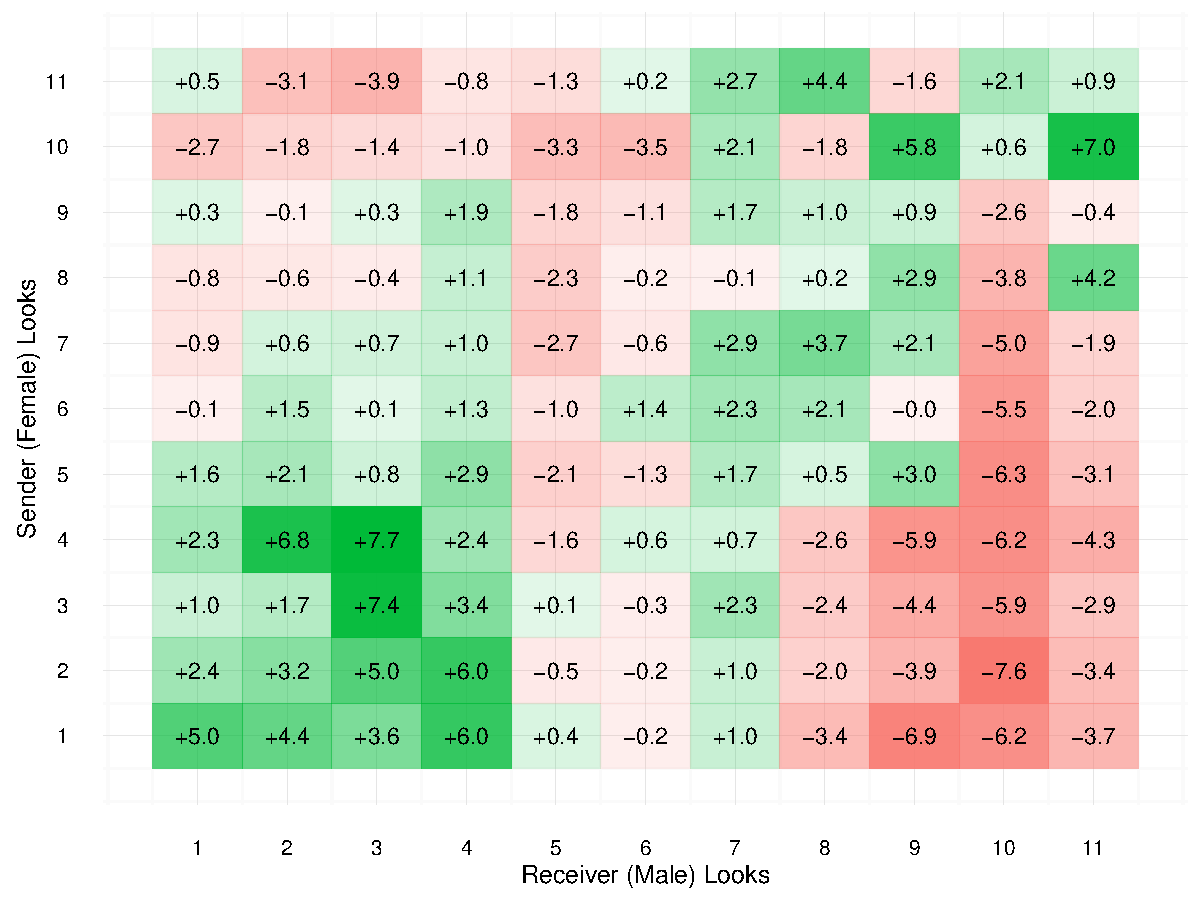
\includegraphics[width=\textwidth]{heatmap_female.pdf}
    \label{fig:heatmap_female}
  \end{subfigure}
  \hfill
  \begin{subfigure}[b]{0.49\textwidth}
    \caption{Relative Preferences of Male Senders}
    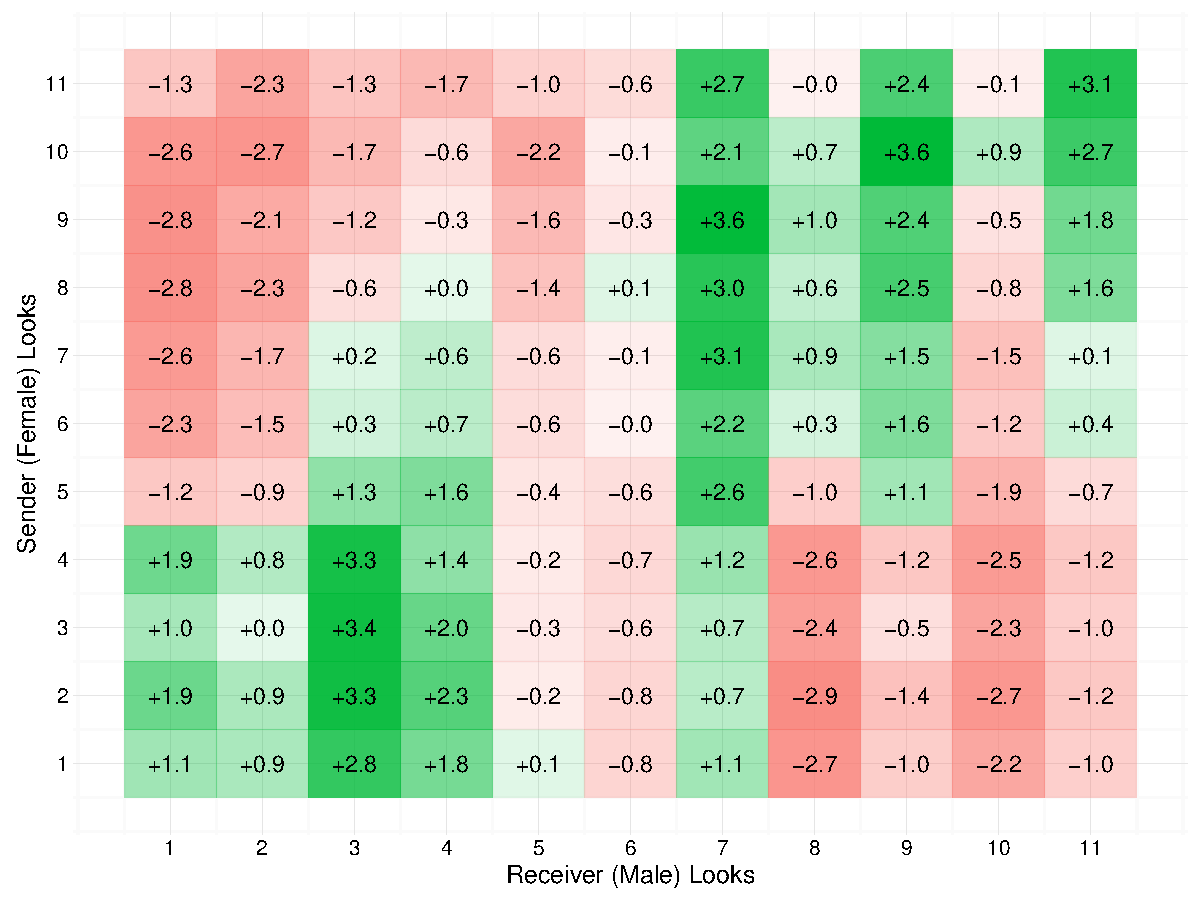
\includegraphics[width=\textwidth]{heatmap_male.pdf}
    \label{fig:heatmap_male}
  \end{subfigure}
\end{figure}

A few random observation:
\begin{itemize}
\item It pays to be an average-looking woman, but not an average-looking man. Conditional on their own ratings, men are slightly more likely to reach out to a woman who is rated  6, while women are slightly less likely to reach out to men who are rated 6. 
\item The pattern reverses for those receivers who are rated slightly above average. Men are less likely to reach out to a woman who is rated a 7, while women are more likely to reach out to a man who is rated a 7.
\item In general, men and women both tend to aim for partners who are rated similar to themselves. This is why we see positive numbers concentrated on the diagonal axis in \cref{fig:heatmap_female} and \cref{fig:heatmap_male}. As a rule, though, men are likely to aim a little higher (or lower!) than women. 
\end{itemize}

We can formalize this last point with a regression:
\[ R_{i,j} = \alpha_j + \beta_j S_{i,j} + \varepsilon_{i,j} \]
where $R_{i,j}$ is the rating of receiver $i$, $S_{i,j}$ is the rating of sender $i$, and $j=\text{\{female,male\}}$. Essentially we are trying to predict the rating of the receiver given the rating of the sender.

The estimated intercept will tell us what is the unconditional expectation for the receivers' ratings. The estimated slope coefficient will tell us the degree to which men or women target those with similar ratings. The higher the coefficient, the more likely it is that senders target similarly rated receivers (i.e. if $\hat{\beta}=1$ then people would only message those who are rated exactly the same as themselves).

% latex table generated in R 3.2.3 by xtable 1.8-2 package
% Mon Apr 25 21:30:19 2016
\begin{table}[ht]
\centering
\caption{Regressing Receiver Looks on Sender Looks} 
\label{tab:receiver_on_sender}
\begin{tabular}{rrrr}
  \hline
 & $\alpha_j$ & $\beta_j$ & R-squared \\ 
  \hline
Female senders & 5.17 & 0.209 & 0.0466 \\ 
  Male senders & 5.94 & 0.159 & 0.0263 \\ 
   \hline
\end{tabular}
\end{table}


For both genders, the unconditional expectation of the receivers' rating is below average (given that the average is a 6). Somewhat surprisingly, women (on average) tend to send messages to men who are slightly \textit{better} looking than they are, while men (on average) send messages to women who are slightly \textit{worse} looking than they are.\footnote{The rating of the average female sender is 5.05 (lower than $\hat{\alpha}_{F}$); the rating of the average male sender is 5.32 (higher than $\hat{\alpha}_{M}$).} Given that the coefficient $\hat{\beta}$ is higher for women than for men, in the aggregate, women are more likely than men to target someone who is rated similarly. Note, however, that the R-squared values for both regressions are very low, so this simple model explains very little of the targeting preferences for either gender.

We can see this most clearly in \cref{fig:dotplot_female} and \cref{fig:dotplot_male}. The volume of messages for a given receiver/sender pair are plotted (bigger dots $\rightarrow$ more messages). Women tend to be a little more discriminating than men, as the bulk of the messages seem to be slightly more concentrated near the diagonal axis. The regression line for each gender is plotted, and we can see that the line for women is a little bit steeper (though not by much!) than the line for the men.

\begin{figure}[!htb]
  \centering
  \caption{}
  \begin{subfigure}[b]{0.49\textwidth}
    \caption{Aggregate Sending Behavior of Females}
    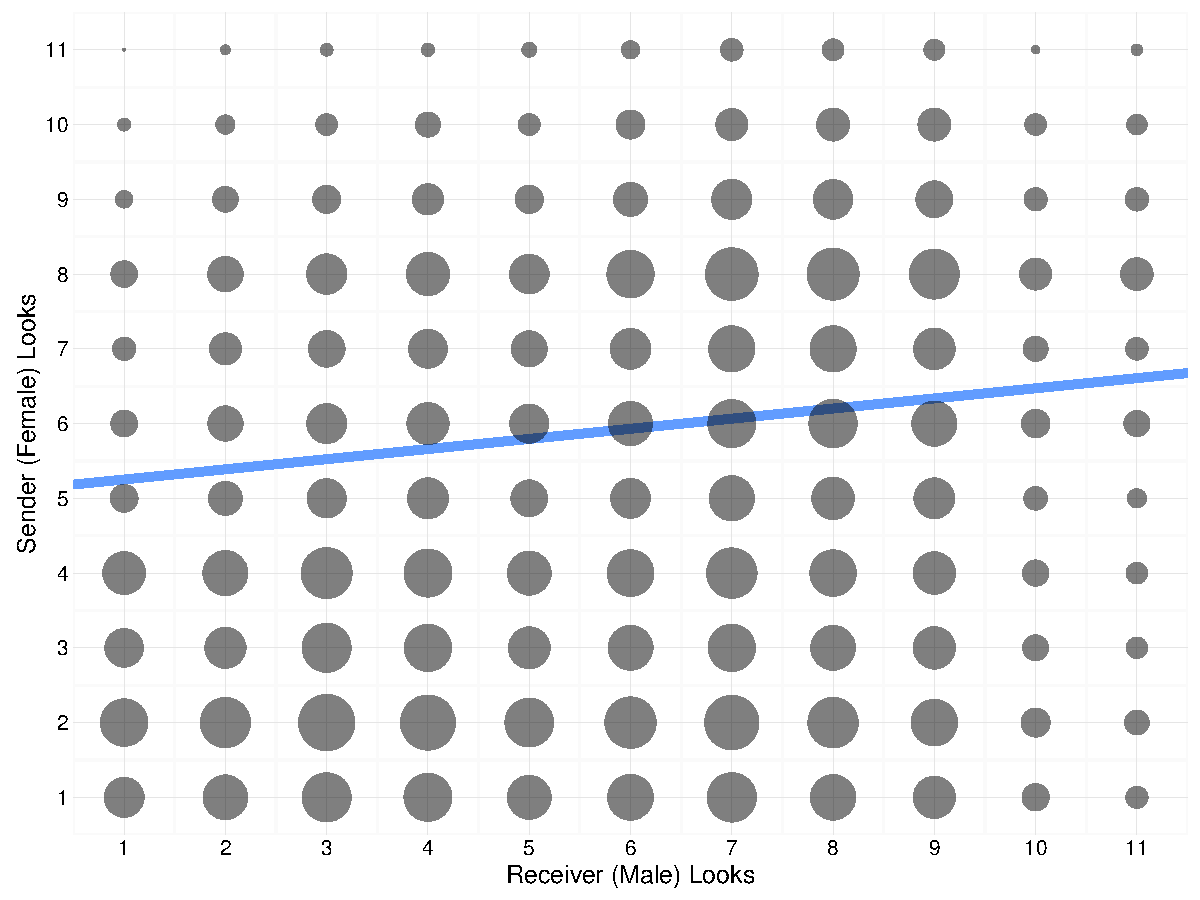
\includegraphics[width=\textwidth]{dotplot_female.pdf}
    \label{fig:dotplot_female}
  \end{subfigure}
  \hfill
  \begin{subfigure}[b]{0.49\textwidth}
    \caption{Aggregate Sending Behavior of Males}
    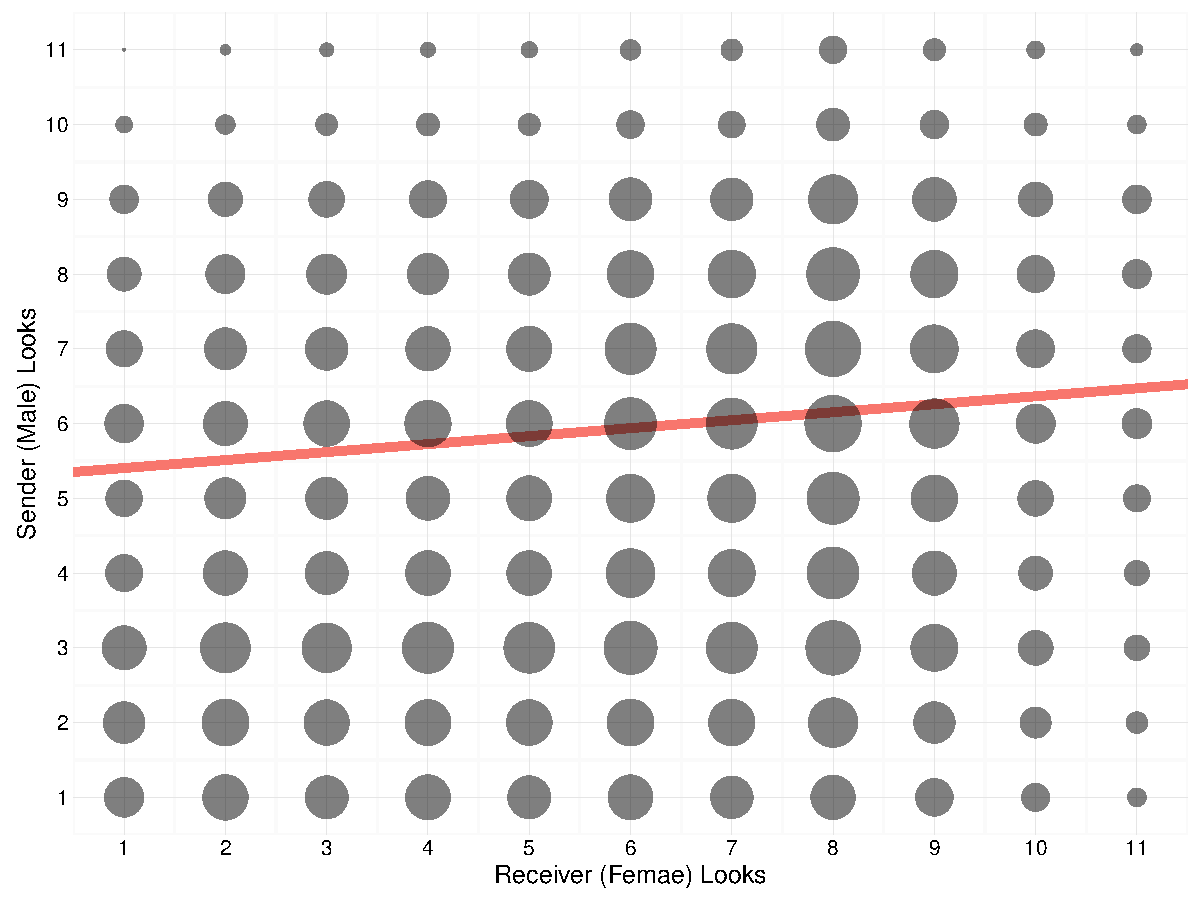
\includegraphics[width=\textwidth]{dotplot_male.pdf}
    \label{fig:dotplot_male}
  \end{subfigure}
\end{figure}


\section{}


\section{}


\section{}

%%%%%%%%%%% BEGIN APPENDIX
\clearpage
\begin{appendices}

\crefalias{section}{appsec}
\section{} \label{app:1}

\end{appendices}

\end{document}

% \input{.tex}

% \begin{figure}[!htb]
%   \centering
%   \caption{}
%   \begin{subfigure}[b]{0.49\textwidth}
%     \caption{}
%     \includegraphics[width=\textwidth]{.pdf}
%     \label{fig:}
%   \end{subfigure}
%   \hfill
%   \begin{subfigure}[b]{0.49\textwidth}
%     \caption{}
%     \includegraphics[width=\textwidth]{.pdf}
%     \label{fig:}
%   \end{subfigure}
% \end{figure}

% \begin{figure}[!htb]
%   \centering
%   \caption{}
%   \includegraphics[scale=.5]{.pdf}
%   \label{fig:}
% \end{figure}